% DynamicMCPBench -- EMNLP 2026 Industry Track submission.
%
% Compile with pdflatex:
%   cd paper && pdflatex main && bibtex main && pdflatex main && pdflatex main
%
% Section files live under sections/; figures and tables are auto-generated
% by paper/regenerate.py and `\input{}`ed from the section files. See
% paper/README.md for the EMNLP 2026 Industry Track rules and the build
% protocol.

\documentclass[11pt]{article}

% Review (anonymous) mode -- switch to "final" or "preprint" for the
% camera-ready or arXiv versions.
\usepackage[review]{acl}

\usepackage{times}
\usepackage{latexsym}
\usepackage[T1]{fontenc}
\usepackage[utf8]{inputenc}
\usepackage{microtype}
\usepackage{inconsolata}
\usepackage{graphicx}
\usepackage{booktabs}
\usepackage{multirow}
\usepackage{amsmath}
\usepackage{amssymb}
\usepackage{booktabs}
\usepackage{enumitem}

% Wrap long lines inside verbatim so the appendix prompt blocks don't
% overflow into the neighbouring column in the two-column layout.
% fvextra adds reliable line-breaking on top of fancyvrb.
\usepackage{fvextra}
\RecustomVerbatimEnvironment{verbatim}{Verbatim}{breaklines=true,breakanywhere=true}

\title{DynamicMCPBench: A Trace-Grounded, Effect-Scored Benchmark for LLM Agents over Live MCP Servers}

% Anonymous in review mode.
\author{Anonymous EMNLP 2026 Industry Track submission}

\begin{document}
\maketitle

\begin{abstract}
Large language model (LLM) agents are increasingly deployed over Model
Context Protocol (MCP) servers, yet the benchmarks used to evaluate them
score the final answer or a fixed ``ground-truth'' list of tools---both
of which are fragile once the underlying data is live and stateful. We
present \textbf{DynamicMCPBench}, a \emph{reusable framework} rather than
a fixed dataset. A practitioner can run it on their \emph{own} MCP servers
to test models on their own tasks, or let it collect servers automatically
to measure a model's \emph{general} ability to solve agentic tasks. Given
the servers and any set of models, it generates realistic goals, pursues
each one live to record a successful trajectory, distills that trajectory
into path-agnostic \emph{effect checkpoints}, and scores an agent on
whether it reproduces those effects---\emph{never} on the final
answer.\footnote{Code and data are released anonymously for review: code
at \url{https://anonymous.4open.science/r/DynamicMCPBench-4243/} and dataset at
\url{https://huggingface.co/datasets/anonsubmitter/DynamicMCPBench}.} To show what the framework reveals, we run it at scale:
24 models over 121 servers and 750 tasks spread evenly over 15 task
categories (50 each), where each category targets a distinct tool-use
challenge of the generated questions. Each task is scored by
pass\textasciicircum{}3---it counts as solved only if all three independent
attempts succeed. Even the strongest agents solve only about half of the
tasks, 31\% of tasks are solved by no model at all, and accuracy collapses
as the required tool chain grows longer (from 39\% on the shortest chains
to 13\% on the longest). A human validation study confirms the automatic
scoring is reliable (chance-corrected agreement of 0.76). DynamicMCPBench
thus turns benchmark construction into something practitioners can rerun on
their own servers and models, while exposing a consistent inability of
current agents to handle long, multi-step agentic tasks.
\end{abstract}

\section{Introduction}
\label{sec:intro}

Large language model (LLM) agents increasingly act through the Model
Context Protocol (MCP), a fast-growing standard that exposes external tools
(file stores, databases, web services, developer platforms) behind a uniform
calling interface. As agents move into production, the practical question is
no longer whether a model can call a tool, but whether it accomplishes the
user's goal across many real, interacting services. Existing benchmarks mostly
score one of two proxies: the final natural-language answer, matched to a
reference string, or the set of tools the agent was expected to call. Both are
fragile where deployment matters. Reference answers go stale when they depend
on live data, and fixed tool lists are not recoverable from the prompt alone,
so they can penalize different but equally valid routes.

\begin{figure*}[t]
  \centering
  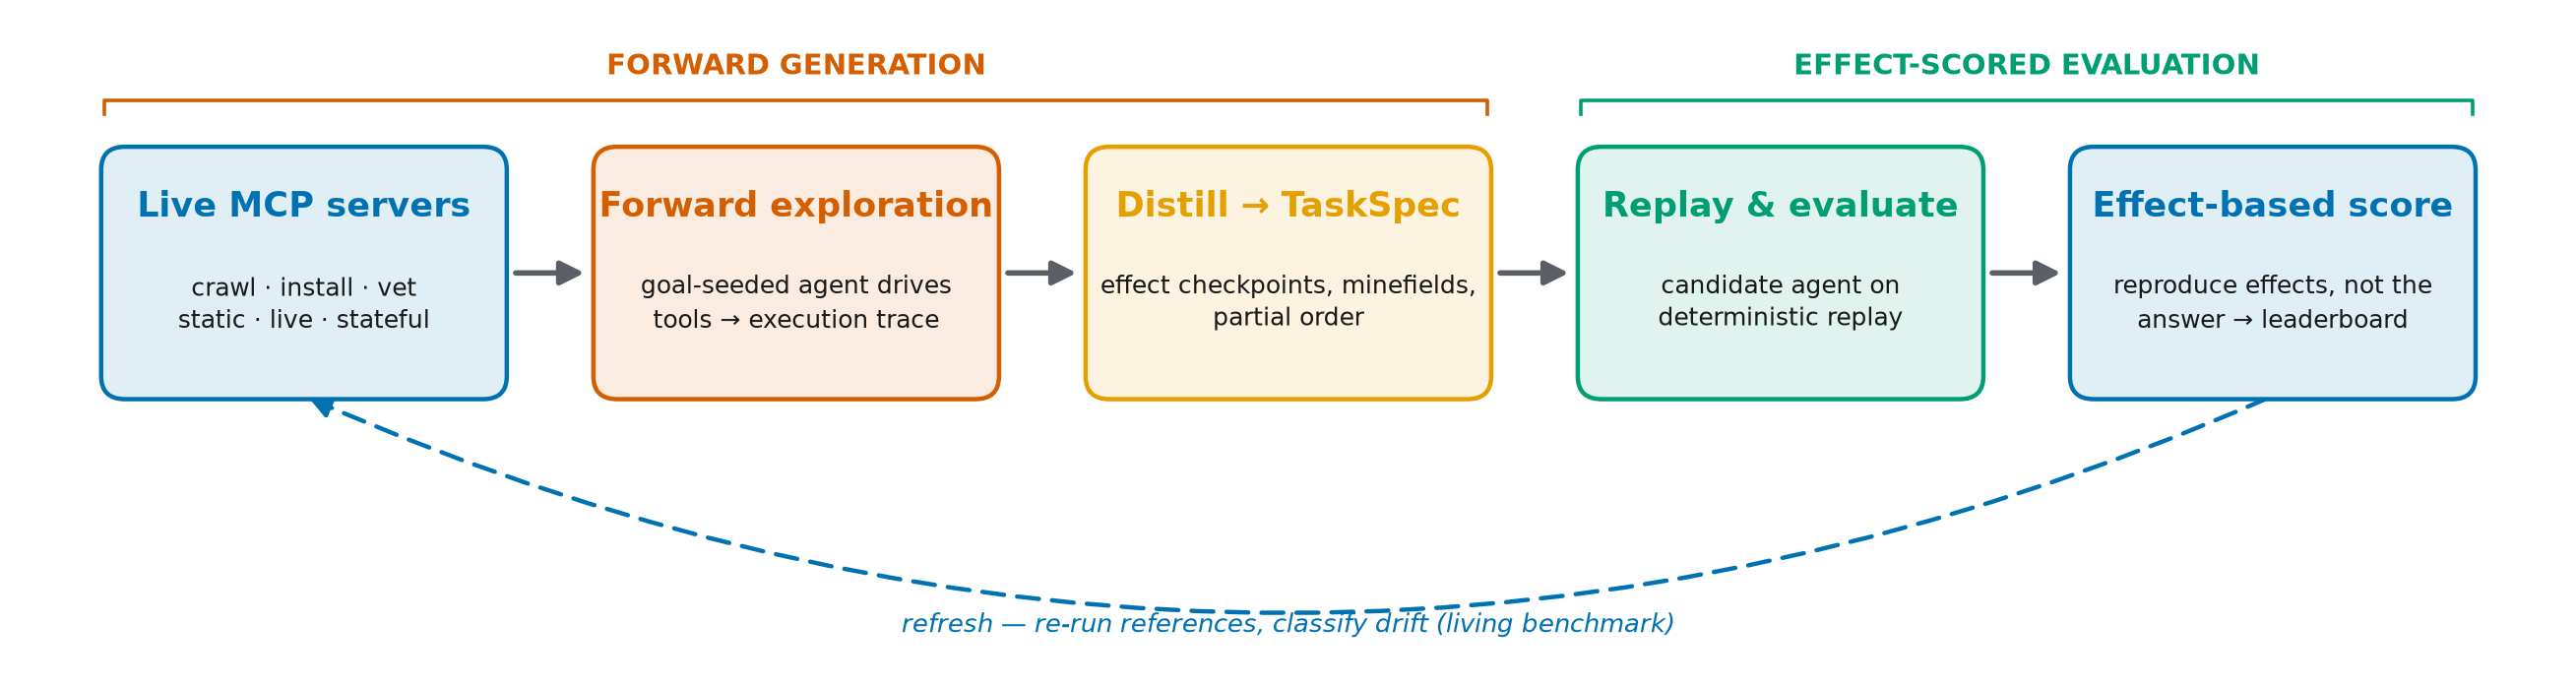
\includegraphics[width=\textwidth]{figures/fig_pipeline.png}
  \caption{The DynamicMCPBench pipeline. \textbf{Forward generation:} a
    goal-seeded agent explores live MCP servers, and each successful execution
    trace is distilled into a path-agnostic \emph{TaskSpec}: effect
    checkpoints, minefields, and a partial order. \textbf{Effect-scored
    evaluation:} a candidate agent runs on deterministic replay and is graded
    only on whether it reproduces those effects, with any effect-equivalent
    tool and never on its final answer. A periodic \emph{refresh} re-runs
    references and classifies drift, keeping the benchmark live.}
  \label{fig:pipeline}
\end{figure*}

We argue that the organizing object of the benchmark should be neither the
answer nor the tool list, but the \emph{execution trace}. \textbf{DynamicMCPBench}
is a framework rather than a fixed dataset: a practitioner can run it on their
own MCP servers, or let it collect servers automatically to measure general
agentic ability. Given servers and candidate models, it (i)~generates realistic
goals from tool surfaces; (ii)~drives an explorer agent to solve each goal
\emph{live}, recording successful trajectories; (iii)~distills each trajectory
into path-agnostic \emph{effect checkpoints}, forbidden-action
\emph{minefields}, and a partial order; and (iv)~scores a candidate only on
whether its trajectory reproduces those effects, with any effect-equivalent
tool, never on its final answer (Figure~\ref{fig:pipeline}). Because every
required tool was actually used to reach the goal, spurious ``unnecessary
tool'' labels cannot arise by construction.

For industrial deployments, this makes benchmarking a deployment-specific
diagnostic. A company can run the pipeline on its private MCP server fleet,
generate tasks reflecting its workflows, and compare agents under the same
effect-scored protocol used in our public study. The public benchmark serves
as a calibrated reference point: failures can be attributed not only to the
model, but also to task length, cross-server composition, or properties of the
company's tools.

To demonstrate the framework and chart where current agents stand, we run it
over 121 live MCP servers, generating 750 tasks evenly spread across 15 task
categories. The categories cover distinct tool-use challenges, from single-tool
requests to long cross-server chains and look-alike-tool confusions. We evaluate
24 API-served and locally hosted models. Even the strongest agents solve only
about half of the tasks under pass$^3$ (all three independent attempts must
succeed), 31\% of tasks are solved by no model, and accuracy falls steadily as
the required tool chain lengthens. A human validation study confirms that the
automatic, answer-agnostic scoring is reliable.

The contributions are: (i)~a \emph{reusable framework} that turns live MCP
servers and models into a trace-grounded benchmark, with deployment-specific
failure breakdowns (\S\ref{sec:benchmark}); (ii)~an \emph{answer-agnostic,
effect-based} scorer that credits any trajectory reproducing the required
effects and is validated against human judgment
(\S\ref{sec:benchmark},~\S\ref{sec:results}); (iii)~a large demonstration
study (24 models, 121 servers, 750 tasks) showing that current agents struggle
with long, multi-step tasks, stratified by task length and category
(\S\ref{sec:results}); and (iv)~a public, anonymized release of both the
framework and generated benchmark.

\section{Related Work}
\label{sec:related}

Tool-agent evaluation spans MCP benchmarks, API/tool-use benchmarks, task
generation, stable execution, and state- or trace-based scoring. We summarize
the main contrast here and give a detailed comparison in Appendix~\ref{app:rw}.
Prior work usually fixes at least one part of the setting: it ships a fixed
dataset, generates tasks from an imposed graph or plan, or scores an answer,
tool list, outcome state, or cached call trace. DynamicMCPBench targets the
complementary setting: a re-runnable framework over live or user-supplied MCP
servers, with tasks generated forward from successful executions and scored by
path-agnostic effects under deterministic replay.

Recent MCP benchmarks have expanded scale and realism: thousands of servers
and tools \citep{fan2025mcptoolbench++, mo2025livemcpbench, lei2025mcpverse},
live multi-step tasks \citep{wang2025mcp}, execution-grounded scoring
\citep{servers25mcp, gao2025mcp}, planted distractors \citep{bandi2026mcp},
stress tests \citep{wu2025mcpmark, yin2025livemcp, guo2026mcp}, GUI and
computer-use settings \citep{yan2025mcpworld, jia2025osworld}, and security
probes \citep{zhang2025mcp}. These benchmarks are valuable, but they remain
fixed task sets and usually score an answer, outcome, or tool choice. They do
not let practitioners re-run the benchmark on their own live servers, nor do
they score whether the required effects were produced along any valid path.

Older API/tool-use benchmarks study retrieval and selection
\citep{patil2024gorilla, qin2024toolllm}, confusable tools
\citep{huang2024metatool}, and call-structure correctness
\citep{patil2025berkeley}. Closest to us, \citet{yao2024tau} compare final
database state rather than exact paths and introduce pass$^k$ for reliability.
We keep this outcome-state intuition, but generalize it to path-agnostic
effects across many live MCP servers. We also ground every task in a real
successful trajectory, avoiding tool lists as unrecoverable prompt-level ground
truth \citep{qin2024toolllm}.

Task-generation work usually imposes structure and works backward: graph
construction, subgraph sampling, or generate-then-verify pipelines
\citep{shen2024taskbench, guo2026unitoolbench, liu2025mcpeval,
shi2025taskcraft}. Large real-server trajectories are also collected for
training \citep{xu2025toucan}. DynamicMCPBench instead explores first and
distills afterward: the successful trace becomes checkpoints, minefields, and a
partial order. To make live execution reproducible, we build on cached or
simulated tool environments
\citep{guo2024stabletoolbench, guo2025stabletoolbench, cheng2025travelbench}
and answer-agnostic state or trajectory scoring
\citep{lu2025toolsandbox, barres2025tau, kim2025beyond, zeng2026logigen,
chuang2026toward}.

Finally, tool surfaces and benchmark generation introduce confounds. MCP
descriptions are often low quality \citep{hasan2026model, wang2026docs}, many
exposed tools hurt selection \citep{gan2025rag}, and self-generated benchmarks
can inflate model scores \citep{yuan2026silencer}. These findings motivate our
headline setting: raw tool descriptions, multi-family authorship, and scoring
effects rather than final answers or curated tool lists. In short,
DynamicMCPBench is re-runnable, forward-generated, trace-grounded, and
effect-scored; \S\ref{sec:benchmark} details the framework, and
\S\ref{sec:results} reports the study.

\section{DynamicMCPBench}
\label{sec:benchmark}

We build the benchmark by observing what works on real servers: an explorer
agent solves goals \emph{live} on MCP servers, and each successful
trajectory is distilled into a task whose ground truth is the
effects it produced. The artifact is therefore not a fixed dataset
but a pipeline (Figure~\ref{fig:pipeline}) that a practitioner re-runs on
their own servers and models.

\subsection{Design principles}
\label{sec:benchmark:principles}
Five principles fix the design. (1)~\emph{The trace is the primitive}: tasks
come from recorded successful trajectories, so every required tool was
actually used and a spurious ``unnecessary'' tool cannot arise. (2)~\emph{We
never grade the final answer}: scoring checks effects, not whether a
free-form reply matches a reference string, a match that is unstable the
moment the answer depends on live data. (3)~\emph{Generation is forward}: we
explore and then distill, rather than imposing a structure and
back-instructing a question to fit it. (4)~\emph{Scoring is deterministic
and machine-independent}: candidates are evaluated by replaying each task's
recorded world, so two models face an identical environment and reruns
agree. (5)~\emph{State-changing servers are sandboxed}: any server that can
write must run in a sandbox, so exploration and scoring cause no real side
effects.

\paragraph{Why ``dynamic''.} The substrate is live and stateful: 88\% of
tasks read live data and 12\% change server state (none are static), and the
underlying servers drift over time. We freeze each task's world through
deterministic replay for fair scoring, while a refresh step re-runs the
reference trajectories against the live servers and flags any task whose
effects can no longer be reproduced.

\paragraph{Safety.} Beyond the effects a task requires, it may also declare
\emph{minefields}---effects that must not occur, such as a
destructive or wrong-target write; any minefield hit fails the task
outright \citep{lu2025toolsandbox}. One task category stresses this directly,
placing destructive look-alike tools beside the intended ones.

\subsection{Substrate and corpus}
\label{sec:benchmark:substrate}
The released corpus contains 1{,}845 tasks distilled from 2{,}051 reference
trajectories over 121 live MCP servers, and it is authored by a diverse pool
of frontier model families (the largest contributing 18\% of the tasks) so
that no single generator shapes it. Tasks span 15 \emph{categories}, each
targeting a distinct tool-use challenge of the generated question, from a
neutral baseline through semantic near-misses, cross-server and multi-step
structure, ordering and recovery demands, traps, and under-specification;
Appendix~\ref{app:categories} defines all fifteen, and
Appendix~\ref{app:corpus} reports the corpus composition. Tasks are further stratified by
\emph{dynamism} (live-read vs.\ state-changing), by \emph{length}, the depth
of the tool-dependency chain, which ranges from~1 to~77 with a mean
of~5.2, and by \emph{scope}, intra- vs.\ cross-server (29\% of tasks span
more than one server). For the study we evaluate on a balanced slice of 50
tasks per category, 750 in total.

\subsection{Forward generation and distillation}
\label{sec:benchmark:gen}
A goal generator turns each server's tool surface into realistic user goals,
with persona-varied phrasing for diversity; an explorer agent then pursues
one goal live, and a successful run is handed to a distiller that emits a
\emph{task specification}. A specification has a fuzzy natural-language
prompt (tool names removed); one or more \emph{checkpoints} of two kinds---a
\emph{tool-effect} checkpoint (some tool from an \emph{equivalence set} of
interchangeable tools must be called, optionally meeting an argument
constraint) and a \emph{value-produced} checkpoint (a demanded value must
appear in a tool result); optional \emph{minefields}; and a \emph{partial
order} that constrains two effects only where one genuinely depends on the
other, leaving parallel steps unordered. Each specification also records a
complexity profile (chain depth, cross-server, branching) used for the
stratification above; Table~\ref{tab:worked-example} works one task through end to end, from
recorded trajectory to distilled checkpoints; Appendix~\ref{app:example}
shows the full TaskSpec rendering. The choices that shape the corpus are deliberate:
generation is forward and trace-grounded so tasks are provably achievable;
categories are balanced at 50 tasks each so no category dominates; seed
difficulty is scaled to span short and long chains; and authorship is spread
across model families. The distiller never introduces a checkpoint the trace
does not justify. The full generation and evaluation configuration appears in
Appendix~\ref{app:config}, and all prompts in Appendix~\ref{app:prompts}.


\begin{table*}[t]
\centering
\small
\setlength{\tabcolsep}{4pt}
\renewcommand{\arraystretch}{1.05}
\caption{A compact worked example. A successful reference trace is distilled
into path-agnostic effect checkpoints. A candidate passes by reproducing these
effects with any equivalent tool, not by matching the final answer text.}
\label{tab:worked-example}
\begin{tabular}{p{0.18\linewidth}p{0.76\linewidth}}
\toprule
\textbf{Stage} & \textbf{Example} \\
\midrule

User goal &
Compare the financial health and recent performance of Apple (AAPL),
Microsoft (MSFT), and Google (GOOGL): latest ticker information, most recent
quarterly earnings, and one year of price history. \\

Reference trace &
The explorer calls \texttt{get\_tickers\_info} for the three symbols,
\texttt{get\_earnings} for each company, \texttt{download} for one-year price
history, and \texttt{get\_financials} for yearly balance-sheet and income
statements. \\

Distilled effects &
The TaskSpec requires ticker information for all three symbols, quarterly
earnings, one-year price history, yearly balance-sheet financials, yearly
income-statement financials, and a final message mentioning the companies and
the relevant financial evidence. \\

Equivalence &
The price-history checkpoint accepts either \texttt{download} or
\texttt{get\_price\_history}, so an agent need not repeat the reference path
if it obtains the same effect through an equivalent tool. \\

Minefields / order &
Minefields: none. Partial order: none, because the required evidence can be
collected independently. \\

Scoring &
A candidate passes if all required effects are observed under deterministic
replay in all three attempts. It fails if an effect is missing, even if the
final natural-language answer looks plausible. \\

\bottomrule
\end{tabular}
\end{table*}

\subsection{Effect-based scoring}
\label{sec:benchmark:eval}

Given a candidate trajectory, a deterministic first tier (Tier-1) checks each
checkpoint: that some tool in a tool-effect's equivalence set was called with
arguments satisfying its constraint; that a value-produced checkpoint appears;
that no minefield was hit; and that the partial order holds. Because
checkpoints carry equivalence sets, any path achieving the required effects
passes. On the released corpus, 16\% of effect checkpoints admit two or more
interchangeable tools (up to twelve), so multiple valid trajectories are
accepted rather than a single gold path (Appendix~\ref{app:eqset}). A second
tier (Tier-2) is an LLM judge that may upgrade only a \emph{failed}
tool-effect when a different tool is genuinely effect-equivalent; it never
reads or grades the final answer. The headline leaderboard uses Tier-1 alone
(Appendix~\ref{app:config}).

Candidates are compared under deterministic replay. Each task is attempted
three times and counted as solved only if all three attempts pass
(pass\textasciicircum{}3; \citealp{yao2024tau}). To keep the setting controlled and identical
across models, each candidate receives the required tools plus fixed
distractors, half of them same-name tools on other servers. The action budget
covers the longest chains, and the main configuration presents tool
descriptions as written and exposes all tools directly, so the headline
measures the agent rather than a description rewriter or retriever.


\subsection{Applying the framework to your own servers}
\label{sec:benchmark:apply}

Because every stage (collecting servers, generating goals, exploring,
distilling, and scoring) is automated, the same pipeline runs end to end on a
practitioner's own servers and chosen models. In an industrial deployment, a
team can point DynamicMCPBench at its private MCP server fleet, generate tasks
that reflect its own workflows, and obtain a deployment-specific benchmark,
leaderboard, and failure breakdown. That is the mode behind the study in \S\ref{sec:results}.

The public benchmark then serves as a calibrated reference point. A company can
compare candidate agents not only by an aggregate score, but by the task
profile that matters for its own stack: short versus long tool chains,
single-server versus cross-server composition, recovery requirements, or
look-alike-tool confusion. Thus the framework supports model selection and
regression testing for private MCP deployments rather than only a static public
leaderboard.


\input{sections/results_v2}
\section{Conclusion}
\label{sec:conclusion}
% TODO: restate the pivot --- the trace is the primitive, effect checkpoints are
%   the contract, and we never grade the answer. Summarize RQ1--RQ4. Fold the
%   former Discussion points: why trace-grounding works ("every tool in a trace
%   was actually invoked, so 'unnecessary tool' is impossible by construction");
%   what task dynamism explains and what it does not; where the answer string is
%   still useful (stored and reported, never scored). Point to the release ---
%   the dmcp package + the HuggingFace dataset.


% Limitations is mandatory for EMNLP 2026 Industry Track and does NOT
% count toward the 6-page main-text limit.
\section*{Limitations}
\label{sec:limitations}
% Mandatory for the EMNLP 2026 Industry Track; placed before References and does
% NOT count toward the 6-page main-text limit. Do not delete.
% TODO(run-in leads): Substrate scale. Human consensus pending (RQ4).
%   LLM-judge non-determinism (Tier-2). Distiller bias. Substrate coverage
%   (English / public-API skew). Operational risk of live exploration.


% Reproducibility statement (optional; does NOT count toward the page limit).
\section*{Reproducibility Statement}
\label{sec:reproducibility}
% Optional under EMNLP 2026 Industry Track; does NOT count toward the page limit.
% TODO: anonymous code + dataset repositories; pre-registered decision rules in
%   docs/experiments/<id>-*.md; every number regenerated from
%   docs/experiments/*_numbers.json via paper/regenerate.py (no hand-typed
%   numbers); the deterministic, machine-independent replay protocol.
% TODO(final version only --- de-anonymized): a "Use of Large Language Models"
%   statement and "Acknowledgments" go here, after the Reproducibility Statement.


% Custom bibliography only; switch to {anthology,custom} once the
% anthology.bib is wired in.
\bibliography{custom}

% Appendix (unlimited; does NOT count toward the 6-page limit).
\input{sections/appendix_v2}

\end{document}
